\documentclass[11pt,letterpaper,twocolumn]{article}

\usepackage{graphicx}
\usepackage{hyperref}
\topmargin=-1in
\evensidemargin=0in
\oddsidemargin=0in
\textwidth=6.5in
\textheight=9.0in
\headsep=0.25in

\begin{document}

\title{Hoja de trabajo No.1}
\author{Sébastien Escobar}
\maketitle

\subsection*{Informatica 1}
\renewcommand{\abstractname}{Ejercicio No.2 Abstracción}

\begin{abstract}
Considerando un dado de seis caras, el cual se coloca en una superficie y solo puede rotar 90 grados en cualquiera de sus 4 lados.
\\
\\Se hace una modelacion del dado y sus transiciones de estado como un grafo.
Para ello se conforma el conjunto de nodos sobre el grafo:
\subsection*{Nodos}
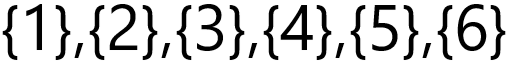
\includegraphics[height=0.8cm]{nodos}
\\
\\Sean los nodos las 6 posibilidades en las cuales podria caer el dado segun el tiro que se haga. Por otro lado los vertices, que se presentan a continuación son las parejas ordenadas por las cuales el dado puede moverse. Hasta llegar a su destino siendo este el nodo final. Y tomando 1 como el incial.
\subsection*{Vertices}
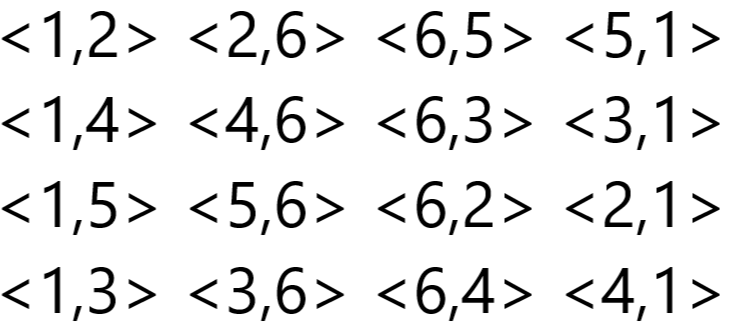
\includegraphics[height=3.5cm]{vertices}

\subsection*{Simulación utilizando un grafo }

\end{abstract}

\renewcommand{\abstractname}{Ejercicio No.3}
\begin{abstract}
\subsection*{¿Que estructura de datos podria representar un lanzamiento de dados?}
Un grafo en el cual existe un camino con dos nodos especiales uno de los cuales comienza en
"1" y posee dos ciclos que viaja a través de vértices con los cuales se conectan a cualquier
posibilidad del dado siendo este el segundo nodo. El camino a cuál sea el número (aleatorio)
al cual se quiere llegar, está determinado por un conjunto de vértices antes de llegar al mismo.
\subsection*{¿Que algoritmo podriamos utilizar para generar dicha estructura?}
Podríamos utilizar el algoritmo de Búsqueda de Uniones. Ya que se colocan nodos para los
que exista un camino en una misma clase de equivalencia Antes de agregar un vértice [x,y],
revisar que X y Y no se encuentren en la misma clase de equivalencia.
\subsection*{¿Como nos aseguramos que ese algoritmo siempre produce un resultado?}
Antes de agregar un vertice [1, x], se revisa que x no se encuentre en la misma clase de equivalencia. Se colocan los nodos para los que exista un camino en una misma clase
de equivalencia. Por ultimo se encuentran los vertices que mejor se acoplen para llegar eficientemente al segundo nodo. Y así lograr un resultado rapido y eficiente cada vez con este algoritmo.

\end{abstract}

\end{document}

